\documentclass[12pt]{article} 
% Formatting
\tolerance=1000
\usepackage[margin=1.2in]{geometry}


% Custom definitions
% To use this customization file, insert the line "% Custom definitions
% To use this customization file, insert the line "% Custom definitions
% To use this customization file, insert the line "\input{custom}" in the header of the tex file.

% Formatting

\tolerance=1000

% Packages

% \usepackage{amssymb,latexsym}
\usepackage{amssymb,amsfonts,amsmath,latexsym,amsthm}
\usepackage[usenames,dvipsnames]{color}
\usepackage[]{graphicx}
\usepackage[space]{grffile}
\usepackage{mathrsfs}   % fancy math font
% \usepackage[font=small,skip=0pt]{caption}
\usepackage[skip=0pt]{caption}
\usepackage{subcaption}
\usepackage{verbatim}
\usepackage{url}
\usepackage{bm}
\usepackage{dsfont}
\usepackage{extarrows}
\usepackage{multirow}
% \usepackage{wrapfig}
% \usepackage{epstopdf}
\usepackage{rotating}
\usepackage{tikz}
\usetikzlibrary{fit}					% fitting shapes to coordinates
%\usetikzlibrary{backgrounds}	% drawing the background after the foreground

% \usepackage[dvipdfm,colorlinks,citecolor=blue,linkcolor=blue,urlcolor=blue]{hyperref}
\usepackage[colorlinks,citecolor=blue,linkcolor=blue,urlcolor=blue]{hyperref}
%\usepackage{hyperref}
\usepackage[authoryear,round]{natbib}


%  Theorems, etc.

\theoremstyle{plain}
\newtheorem{theorem}{Theorem}[section]
\newtheorem{corollary}[theorem]{Corollary}
\newtheorem{lemma}[theorem]{Lemma}
\newtheorem{proposition}[theorem]{Proposition}
\newtheorem{condition}[theorem]{Condition}
% \newtheorem{conditions}[theorem]{Conditions}

\theoremstyle{definition}
\newtheorem{definition}[theorem]{Definition}
% \newtheorem*{unnumbered-definition}{Definition}
\newtheorem{example}[theorem]{Example}
\theoremstyle{remark}
\newtheorem*{remark}{Remark}
\numberwithin{equation}{section}


% footnote without number
\newcommand\blankfootnote[1]{%
  \begingroup
  \renewcommand\thefootnote{}\footnote{#1}%
  \addtocounter{footnote}{-1}%
  \endgroup
}
\makeatletter
\renewcommand\footnoterule{%
  \kern-3\p@
  \hrule\@width \textwidth
  \kern2.6\p@}
\makeatother

% Document-specific shortcuts
\newcommand{\btheta}{{\bm\theta}}
\newcommand{\bbtheta}{{\pmb{\bm\theta}}}

\newcommand{\commentary}[1]{\ifx\showcommentary\undefined\else \emph{#1}\fi}

\newcommand{\term}[1]{\textit{\textbf{#1}}}

% Math shortcuts

% Probability distributions
\DeclareMathOperator*{\Exp}{Exp}
\DeclareMathOperator*{\TExp}{TExp}
\DeclareMathOperator*{\Bernoulli}{Bernoulli}
\DeclareMathOperator*{\Beta}{Beta}
\DeclareMathOperator*{\Ga}{Gamma}
\DeclareMathOperator*{\TGamma}{TGamma}
\DeclareMathOperator*{\Poisson}{Poisson}
\DeclareMathOperator*{\Binomial}{Binomial}
\DeclareMathOperator*{\NormalGamma}{NormalGamma}
\DeclareMathOperator*{\InvGamma}{InvGamma}
\DeclareMathOperator*{\Cauchy}{Cauchy}
\DeclareMathOperator*{\Uniform}{Uniform}
\DeclareMathOperator*{\Gumbel}{Gumbel}
\DeclareMathOperator*{\Pareto}{Pareto}
\DeclareMathOperator*{\Mono}{Mono}
\DeclareMathOperator*{\Geometric}{Geometric}
\DeclareMathOperator*{\Wishart}{Wishart}

% Math operators
\DeclareMathOperator*{\argmin}{argmin}
\DeclareMathOperator*{\argmax}{argmax}
\DeclareMathOperator*{\Cov}{Cov}
\DeclareMathOperator*{\diag}{diag}
\DeclareMathOperator*{\median}{median}
\DeclareMathOperator*{\Vol}{Vol}
\newcommand{\logit}{\mathrm{logit}}

% Math characters
\newcommand{\R}{\mathbb{R}}
\newcommand{\Z}{\mathbb{Z}}
\newcommand{\E}{\mathbb{E}}
\renewcommand{\Pr}{\mathbb{P}}
\newcommand{\1}{\mathds{1}}
\newcommand{\V}{\mathbb{V}}

\newcommand{\A}{\mathcal{A}}
\newcommand{\C}{\mathcal{C}}
\newcommand{\D}{\mathcal{D}}
\newcommand{\Hcal}{\mathcal{H}}
\newcommand{\I}{\mathcal{I}}
\newcommand{\J}{\mathcal{J}}
\newcommand{\M}{\mathcal{M}}
\newcommand{\N}{\mathcal{N}}
\newcommand{\X}{\mathcal{X}}
\newcommand{\Zcal}{\mathcal{Z}}
\renewcommand{\P}{\mathcal{P}}

\newcommand{\T}{\mathtt{T}}
\renewcommand{\emptyset}{\varnothing}


% Miscellaneous commands
\newcommand{\iid}{\stackrel{\mathrm{iid}}{\sim}}
\newcommand{\matrixsmall}[1]{\bigl(\begin{smallmatrix}#1\end{smallmatrix} \bigr)}

\newcommand{\items}[1]{\begin{itemize} #1 \end{itemize}}

\newcommand{\todo}[1]{\emph{\textcolor{red}{(#1)}}}

\newcommand{\branch}[4]{
\left\{
	\begin{array}{ll}
		#1  & \mbox{if } #2 \\
		#3 & \mbox{if } #4
	\end{array}
\right.
}

% approximately proportional to
\def\app#1#2{%
  \mathrel{%
    \setbox0=\hbox{$#1\sim$}%
    \setbox2=\hbox{%
      \rlap{\hbox{$#1\propto$}}%
      \lower1.3\ht0\box0%
    }%
    \raise0.25\ht2\box2%
  }%
}
\def\approxprop{\mathpalette\app\relax}

% \newcommand{\approptoinn}[2]{\mathrel{\vcenter{
  % \offinterlineskip\halign{\hfil$##$\cr
    % #1\propto\cr\noalign{\kern2pt}#1\sim\cr\noalign{\kern-2pt}}}}}

% \newcommand{\approxpropto}{\mathpalette\approptoinn\relax}





" in the header of the tex file.

% Formatting

\tolerance=1000

% Packages

% \usepackage{amssymb,latexsym}
\usepackage{amssymb,amsfonts,amsmath,latexsym,amsthm}
\usepackage[usenames,dvipsnames]{color}
\usepackage[]{graphicx}
\usepackage[space]{grffile}
\usepackage{mathrsfs}   % fancy math font
% \usepackage[font=small,skip=0pt]{caption}
\usepackage[skip=0pt]{caption}
\usepackage{subcaption}
\usepackage{verbatim}
\usepackage{url}
\usepackage{bm}
\usepackage{dsfont}
\usepackage{extarrows}
\usepackage{multirow}
% \usepackage{wrapfig}
% \usepackage{epstopdf}
\usepackage{rotating}
\usepackage{tikz}
\usetikzlibrary{fit}					% fitting shapes to coordinates
%\usetikzlibrary{backgrounds}	% drawing the background after the foreground

% \usepackage[dvipdfm,colorlinks,citecolor=blue,linkcolor=blue,urlcolor=blue]{hyperref}
\usepackage[colorlinks,citecolor=blue,linkcolor=blue,urlcolor=blue]{hyperref}
%\usepackage{hyperref}
\usepackage[authoryear,round]{natbib}


%  Theorems, etc.

\theoremstyle{plain}
\newtheorem{theorem}{Theorem}[section]
\newtheorem{corollary}[theorem]{Corollary}
\newtheorem{lemma}[theorem]{Lemma}
\newtheorem{proposition}[theorem]{Proposition}
\newtheorem{condition}[theorem]{Condition}
% \newtheorem{conditions}[theorem]{Conditions}

\theoremstyle{definition}
\newtheorem{definition}[theorem]{Definition}
% \newtheorem*{unnumbered-definition}{Definition}
\newtheorem{example}[theorem]{Example}
\theoremstyle{remark}
\newtheorem*{remark}{Remark}
\numberwithin{equation}{section}


% footnote without number
\newcommand\blankfootnote[1]{%
  \begingroup
  \renewcommand\thefootnote{}\footnote{#1}%
  \addtocounter{footnote}{-1}%
  \endgroup
}
\makeatletter
\renewcommand\footnoterule{%
  \kern-3\p@
  \hrule\@width \textwidth
  \kern2.6\p@}
\makeatother

% Document-specific shortcuts
\newcommand{\btheta}{{\bm\theta}}
\newcommand{\bbtheta}{{\pmb{\bm\theta}}}

\newcommand{\commentary}[1]{\ifx\showcommentary\undefined\else \emph{#1}\fi}

\newcommand{\term}[1]{\textit{\textbf{#1}}}

% Math shortcuts

% Probability distributions
\DeclareMathOperator*{\Exp}{Exp}
\DeclareMathOperator*{\TExp}{TExp}
\DeclareMathOperator*{\Bernoulli}{Bernoulli}
\DeclareMathOperator*{\Beta}{Beta}
\DeclareMathOperator*{\Ga}{Gamma}
\DeclareMathOperator*{\TGamma}{TGamma}
\DeclareMathOperator*{\Poisson}{Poisson}
\DeclareMathOperator*{\Binomial}{Binomial}
\DeclareMathOperator*{\NormalGamma}{NormalGamma}
\DeclareMathOperator*{\InvGamma}{InvGamma}
\DeclareMathOperator*{\Cauchy}{Cauchy}
\DeclareMathOperator*{\Uniform}{Uniform}
\DeclareMathOperator*{\Gumbel}{Gumbel}
\DeclareMathOperator*{\Pareto}{Pareto}
\DeclareMathOperator*{\Mono}{Mono}
\DeclareMathOperator*{\Geometric}{Geometric}
\DeclareMathOperator*{\Wishart}{Wishart}

% Math operators
\DeclareMathOperator*{\argmin}{argmin}
\DeclareMathOperator*{\argmax}{argmax}
\DeclareMathOperator*{\Cov}{Cov}
\DeclareMathOperator*{\diag}{diag}
\DeclareMathOperator*{\median}{median}
\DeclareMathOperator*{\Vol}{Vol}
\newcommand{\logit}{\mathrm{logit}}

% Math characters
\newcommand{\R}{\mathbb{R}}
\newcommand{\Z}{\mathbb{Z}}
\newcommand{\E}{\mathbb{E}}
\renewcommand{\Pr}{\mathbb{P}}
\newcommand{\1}{\mathds{1}}
\newcommand{\V}{\mathbb{V}}

\newcommand{\A}{\mathcal{A}}
\newcommand{\C}{\mathcal{C}}
\newcommand{\D}{\mathcal{D}}
\newcommand{\Hcal}{\mathcal{H}}
\newcommand{\I}{\mathcal{I}}
\newcommand{\J}{\mathcal{J}}
\newcommand{\M}{\mathcal{M}}
\newcommand{\N}{\mathcal{N}}
\newcommand{\X}{\mathcal{X}}
\newcommand{\Zcal}{\mathcal{Z}}
\renewcommand{\P}{\mathcal{P}}

\newcommand{\T}{\mathtt{T}}
\renewcommand{\emptyset}{\varnothing}


% Miscellaneous commands
\newcommand{\iid}{\stackrel{\mathrm{iid}}{\sim}}
\newcommand{\matrixsmall}[1]{\bigl(\begin{smallmatrix}#1\end{smallmatrix} \bigr)}

\newcommand{\items}[1]{\begin{itemize} #1 \end{itemize}}

\newcommand{\todo}[1]{\emph{\textcolor{red}{(#1)}}}

\newcommand{\branch}[4]{
\left\{
	\begin{array}{ll}
		#1  & \mbox{if } #2 \\
		#3 & \mbox{if } #4
	\end{array}
\right.
}

% approximately proportional to
\def\app#1#2{%
  \mathrel{%
    \setbox0=\hbox{$#1\sim$}%
    \setbox2=\hbox{%
      \rlap{\hbox{$#1\propto$}}%
      \lower1.3\ht0\box0%
    }%
    \raise0.25\ht2\box2%
  }%
}
\def\approxprop{\mathpalette\app\relax}

% \newcommand{\approptoinn}[2]{\mathrel{\vcenter{
  % \offinterlineskip\halign{\hfil$##$\cr
    % #1\propto\cr\noalign{\kern2pt}#1\sim\cr\noalign{\kern-2pt}}}}}

% \newcommand{\approxpropto}{\mathpalette\approptoinn\relax}





" in the header of the tex file.

% Formatting

\tolerance=1000

% Packages

% \usepackage{amssymb,latexsym}
\usepackage{amssymb,amsfonts,amsmath,latexsym,amsthm}
\usepackage[usenames,dvipsnames]{color}
\usepackage[]{graphicx}
\usepackage[space]{grffile}
\usepackage{mathrsfs}   % fancy math font
% \usepackage[font=small,skip=0pt]{caption}
\usepackage[skip=0pt]{caption}
\usepackage{subcaption}
\usepackage{verbatim}
\usepackage{url}
\usepackage{bm}
\usepackage{dsfont}
\usepackage{extarrows}
\usepackage{multirow}
% \usepackage{wrapfig}
% \usepackage{epstopdf}
\usepackage{rotating}
\usepackage{tikz}
\usetikzlibrary{fit}					% fitting shapes to coordinates
%\usetikzlibrary{backgrounds}	% drawing the background after the foreground

% \usepackage[dvipdfm,colorlinks,citecolor=blue,linkcolor=blue,urlcolor=blue]{hyperref}
\usepackage[colorlinks,citecolor=blue,linkcolor=blue,urlcolor=blue]{hyperref}
%\usepackage{hyperref}
\usepackage[authoryear,round]{natbib}


%  Theorems, etc.

\theoremstyle{plain}
\newtheorem{theorem}{Theorem}[section]
\newtheorem{corollary}[theorem]{Corollary}
\newtheorem{lemma}[theorem]{Lemma}
\newtheorem{proposition}[theorem]{Proposition}
\newtheorem{condition}[theorem]{Condition}
% \newtheorem{conditions}[theorem]{Conditions}

\theoremstyle{definition}
\newtheorem{definition}[theorem]{Definition}
% \newtheorem*{unnumbered-definition}{Definition}
\newtheorem{example}[theorem]{Example}
\theoremstyle{remark}
\newtheorem*{remark}{Remark}
\numberwithin{equation}{section}


% footnote without number
\newcommand\blankfootnote[1]{%
  \begingroup
  \renewcommand\thefootnote{}\footnote{#1}%
  \addtocounter{footnote}{-1}%
  \endgroup
}
\makeatletter
\renewcommand\footnoterule{%
  \kern-3\p@
  \hrule\@width \textwidth
  \kern2.6\p@}
\makeatother

% Document-specific shortcuts
\newcommand{\btheta}{{\bm\theta}}
\newcommand{\bbtheta}{{\pmb{\bm\theta}}}

\newcommand{\commentary}[1]{\ifx\showcommentary\undefined\else \emph{#1}\fi}

\newcommand{\term}[1]{\textit{\textbf{#1}}}

% Math shortcuts

% Probability distributions
\DeclareMathOperator*{\Exp}{Exp}
\DeclareMathOperator*{\TExp}{TExp}
\DeclareMathOperator*{\Bernoulli}{Bernoulli}
\DeclareMathOperator*{\Beta}{Beta}
\DeclareMathOperator*{\Ga}{Gamma}
\DeclareMathOperator*{\TGamma}{TGamma}
\DeclareMathOperator*{\Poisson}{Poisson}
\DeclareMathOperator*{\Binomial}{Binomial}
\DeclareMathOperator*{\NormalGamma}{NormalGamma}
\DeclareMathOperator*{\InvGamma}{InvGamma}
\DeclareMathOperator*{\Cauchy}{Cauchy}
\DeclareMathOperator*{\Uniform}{Uniform}
\DeclareMathOperator*{\Gumbel}{Gumbel}
\DeclareMathOperator*{\Pareto}{Pareto}
\DeclareMathOperator*{\Mono}{Mono}
\DeclareMathOperator*{\Geometric}{Geometric}
\DeclareMathOperator*{\Wishart}{Wishart}

% Math operators
\DeclareMathOperator*{\argmin}{argmin}
\DeclareMathOperator*{\argmax}{argmax}
\DeclareMathOperator*{\Cov}{Cov}
\DeclareMathOperator*{\diag}{diag}
\DeclareMathOperator*{\median}{median}
\DeclareMathOperator*{\Vol}{Vol}
\newcommand{\logit}{\mathrm{logit}}

% Math characters
\newcommand{\R}{\mathbb{R}}
\newcommand{\Z}{\mathbb{Z}}
\newcommand{\E}{\mathbb{E}}
\renewcommand{\Pr}{\mathbb{P}}
\newcommand{\1}{\mathds{1}}
\newcommand{\V}{\mathbb{V}}

\newcommand{\A}{\mathcal{A}}
\newcommand{\C}{\mathcal{C}}
\newcommand{\D}{\mathcal{D}}
\newcommand{\Hcal}{\mathcal{H}}
\newcommand{\I}{\mathcal{I}}
\newcommand{\J}{\mathcal{J}}
\newcommand{\M}{\mathcal{M}}
\newcommand{\N}{\mathcal{N}}
\newcommand{\X}{\mathcal{X}}
\newcommand{\Zcal}{\mathcal{Z}}
\renewcommand{\P}{\mathcal{P}}

\newcommand{\T}{\mathtt{T}}
\renewcommand{\emptyset}{\varnothing}


% Miscellaneous commands
\newcommand{\iid}{\stackrel{\mathrm{iid}}{\sim}}
\newcommand{\matrixsmall}[1]{\bigl(\begin{smallmatrix}#1\end{smallmatrix} \bigr)}

\newcommand{\items}[1]{\begin{itemize} #1 \end{itemize}}

\newcommand{\todo}[1]{\emph{\textcolor{red}{(#1)}}}

\newcommand{\branch}[4]{
\left\{
	\begin{array}{ll}
		#1  & \mbox{if } #2 \\
		#3 & \mbox{if } #4
	\end{array}
\right.
}

% approximately proportional to
\def\app#1#2{%
  \mathrel{%
    \setbox0=\hbox{$#1\sim$}%
    \setbox2=\hbox{%
      \rlap{\hbox{$#1\propto$}}%
      \lower1.3\ht0\box0%
    }%
    \raise0.25\ht2\box2%
  }%
}
\def\approxprop{\mathpalette\app\relax}

% \newcommand{\approptoinn}[2]{\mathrel{\vcenter{
  % \offinterlineskip\halign{\hfil$##$\cr
    % #1\propto\cr\noalign{\kern2pt}#1\sim\cr\noalign{\kern-2pt}}}}}

% \newcommand{\approxpropto}{\mathpalette\approptoinn\relax}







% Packages

% \usepackage{amssymb,latexsym}
\usepackage{amssymb,amsfonts,amsmath,latexsym,amsthm}
\usepackage[usenames,dvipsnames]{color}
\usepackage[]{graphicx}
\usepackage[space]{grffile}
\usepackage{mathrsfs}   % fancy math font
% \usepackage[font=small,skip=0pt]{caption}
\usepackage[skip=0pt]{caption}
\usepackage{subcaption}
\usepackage{verbatim}
\usepackage{url}
\usepackage{bm}
\usepackage{dsfont}
\usepackage{extarrows}
\usepackage{multirow}
% \usepackage{wrapfig}
% \usepackage{epstopdf}
\usepackage{rotating}
\usepackage{tikz}
\usetikzlibrary{fit}					% fitting shapes to coordinates
%\usetikzlibrary{backgrounds}	% drawing the background after the foreground


% \usepackage[dvipdfm,colorlinks,citecolor=blue,linkcolor=blue,urlcolor=blue]{hyperref}
\usepackage[colorlinks,citecolor=blue,linkcolor=blue,urlcolor=blue]{hyperref}
%\usepackage{hyperref}
\usepackage[authoryear,round]{natbib}



\title{Consistency, asymptotic normality, and coverage}
\author{}
\date{}


\begin{document}
\maketitle

\tableofcontents
\blankfootnote{This work is licensed under a \href{http://creativecommons.org/licenses/by-nc-nd/4.0/}{Creative Commons Attribution-NonCommercial-NoDerivatives 4.0 International License}.  Jeffrey W. Miller (2016). \textit{Lecture Notes on Advanced Stochastic Modeling}. Duke University, Durham, NC.}

\vspace{2em}

In the (subjective) Bayesian framework, there is no way to objectively evaluate the performance of a procedure---you assume a particular model, and all your inferences are based on the assumption that the model is correct.  In order to assess a Bayesian procedure, we need to step outside the Bayesian framework. BDA chapter 4 discusses some of the non-Bayesian properties that are often considered when evaluating a procedure. There is also some discussion of connections between non-Bayesian and Bayesian approaches.
I would consider model checking (BDA chapter 6) and assessment of predictive performance (BDA chapter 7) to also fall into the category of non-Bayesian methods of assessment (although some people might argue that these are Bayesian). 
Note: This chapter is more theoretical than most of the material in the course. Also, a word of caution---some of the results in Appendix B of BDA seem to be missing some crucial conditions, and the proofs are very sketchy in places, so I would not recommend using Appendix B as a reference.

%\newpage

\section{Example and counterexample}

\subsection{Example}

First, let's look at a really simple example illustrating posterior consistency and asymptotic normality. Some of the terminology here will be explained in the sections below. Consider the following model:
\begin{align*}
& \theta \sim \Exp(1)\\
& X_1,\ldots,X_n | \theta \sim \Exp(\theta),
\end{align*}
and suppose the true distribution $P_0$ is $\Exp(1)$.  So, the model is correctly specified and the true value of the parameter is $\theta_0 = 1$. The posterior distribution is $\theta | x_{1:n} \sim\Ga(1+n,1+\sum_i x_i)$. As illustrated in Figure \ref{figure:example-1} (top), the posterior density appears to become more Gaussian-like as the sample size $n$ increases, and concentrates near the true value, $\theta_0 = 1$.

Indeed, Figure \ref{figure:example-1} (bottom) indicates that the Kolmogorov--Smirnov (KS) distance\footnote{The Kolmogorov--Smirnov distance between univariate distributions with CDFs $F$ and $G$ is $KS(F,G) = \sup_{x\in\R} |F(x)-G(x)|$.} between the posterior and the ``best'' normal approximation to it (defined here as the normal distribution with the same mean and variance as the posterior) appears to be going to zero as $n$ increases. In other words, the posterior is becoming more normal/Gaussian as $n$ increases.
The fact that the KS distance is going to zero is not merely due to the fact that the posterior is concentrating. The KS distance is invariant under affine transformations of $\theta$, i.e., $$ \sup_{\theta\in\R} |F(\theta)-G(\theta)| = \sup_{\theta\in\R} |F(a \theta + b)-G(a \theta + b)|$$ for any $a\neq 0$, $b\in \R$. So in particular, KS is not dependent on the scale.

\begin{figure}
\begin{center}
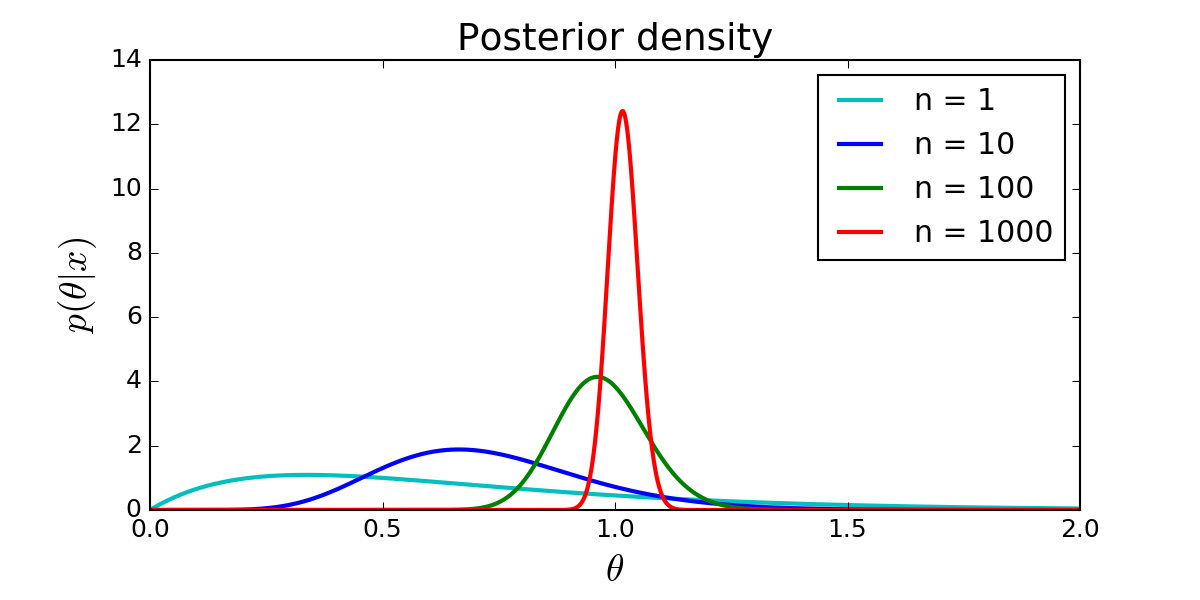
\includegraphics[trim=0 0 0 0, clip, width=0.85\textwidth]{code/ex1-pdf.png}
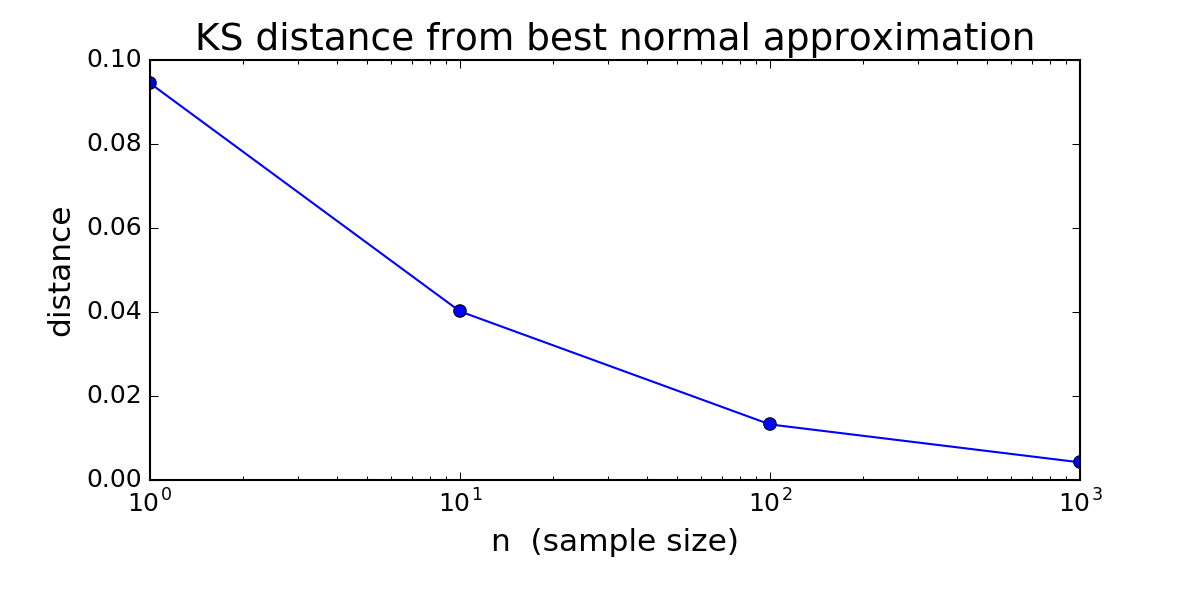
\includegraphics[trim=0 0 0 0, clip, width=0.85\textwidth]{code/ex1-dist.png}
\end{center}
\caption{Empirical demonstration of consistency and asymptotic normality in the exponential example.}
\label{figure:example-1}
\end{figure}


% Model:
%     a ~ Exp(1)
%     x_1,...,x_n|a ~ Exp(a)
% Data: x_1,...,x_n ~ Exp(1)
% The posterior concentrates at the true a and is asymptotically normal.


\subsection{Counterexample}

Now, let's look at an example in which posterior consistency and asymptotic normality do not hold. There are a number of ways in which this can happen, and they do occur in practice, so one needs to be careful. One of the basic requirements is that the parameter be identifiable---that is, that if we knew $P_\theta$ exactly, we could uniquely recover $\theta$  (i.e., if $\theta \neq \theta'$ then $P_\theta \neq P_{\theta'}$). To illustrate this with a very simple example, consider the model:
\begin{align*}
& a,b\sim \Exp(1)\\
& X_1,\ldots,X_n | a,b\sim \Exp(a b),
\end{align*}
and suppose the true values of the parameters are $a_0 = 1$ and $b_0 = 1$, so that the true distribution $P_0$ is $\Exp(1)$. Note that any values of $a$ and $b$ such that $a b = 1$ will give rise to a distribution that matches $P_0$, so if we define $\theta = (a,b)$, then $\theta$ is not identifiable. To see what happens if we sample from the posterior, Figure \ref{figure:counterexample} shows $10^5$ Gibbs samples, for each $n\in \{1,10,100,1000 \}$.

\begin{figure}
\begin{center}
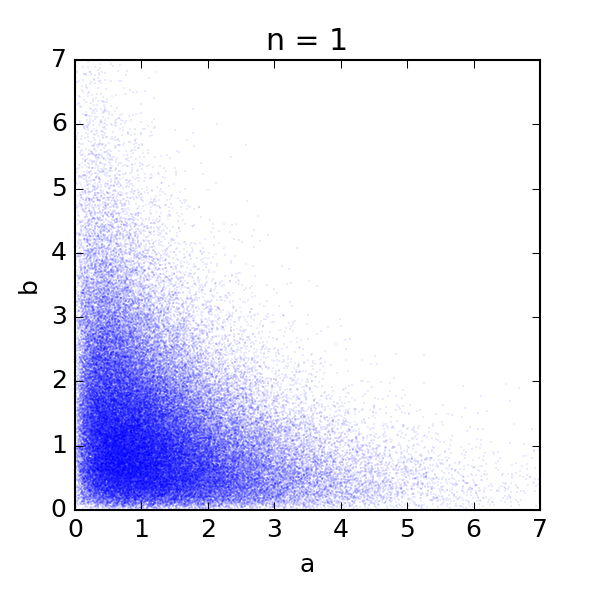
\includegraphics[trim=0 0 0 0, clip, width=0.49\textwidth]{code/ex2-n=1.png}
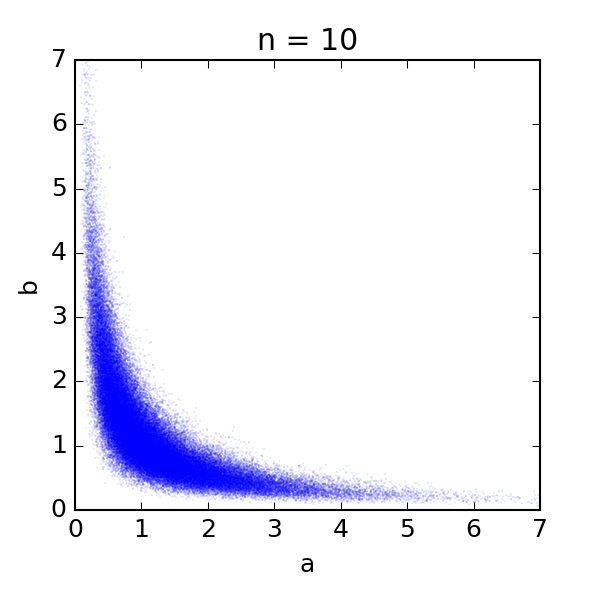
\includegraphics[trim=0 0 0 0, clip, width=0.49\textwidth]{code/ex2-n=10.png}\\
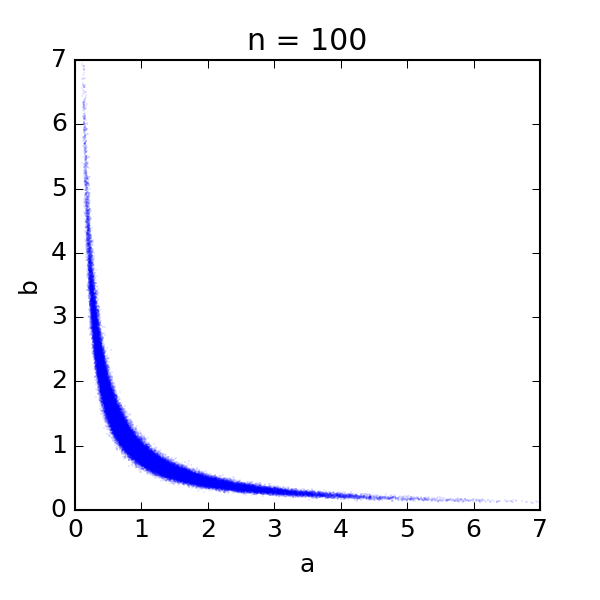
\includegraphics[trim=0 0 0 0, clip, width=0.49\textwidth]{code/ex2-n=100.png}
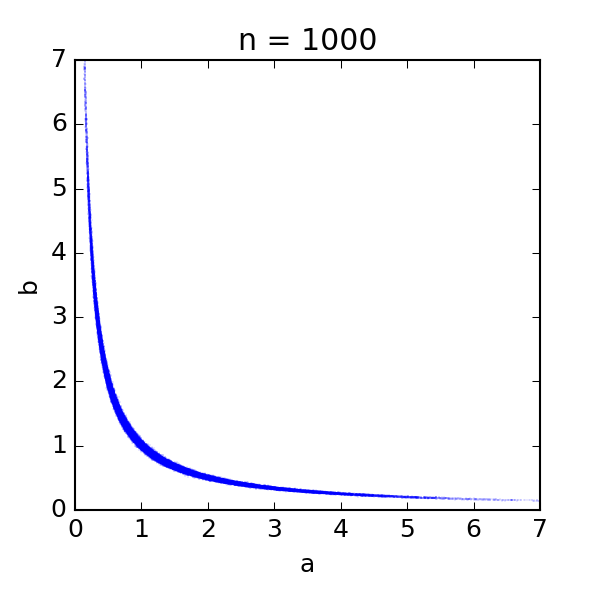
\includegraphics[trim=0 0 0 0, clip, width=0.49\textwidth]{code/ex2-n=1000.png}
\end{center}
\caption{Example in which consistency and asymptotic normality fail due to a lack of identifiability.}
\label{figure:counterexample}
\end{figure}

Note that the posterior is concentrating on the curve satisfying the equation $a b = 1$. However, it is not concentrating at any particular point on the curve, and it is far from normal/Gaussian.
Incidentally, this also serves as an example in which Gibbs sampling mixes poorly when $n$ is large. (Why?)



\section{Consistency}

In the frequentist setting, consistency and asymptotic normality are two basic properties of estimators. In the Bayesian setting, we also consider consistency and asymptotic normality of posterior distributions, which, while similar, are slightly different than the corresponding properties of estimators.

\subsection{Consistency of estimators}

Roughly speaking, an estimator $\hat\beta_n$ of a quantity of interest $\beta$ is said to be \textit{consistent} if $\hat\beta_n \to \beta$ as $n\to\infty$, in other words, if it is guaranteed to converge to the true value. What exactly does this mean? From the frequentist perspective, the observed data $X_{1:n}$ are viewed as random variables generated from some unknown ``true'' distribution $P_0$.  Since $\hat\beta_n$ is a function of the observed data $X_{1:n}$---often denoted by writing $\hat\beta_n = \hat\beta_n(X_{1:n})$---it follows that $\hat\beta_n$ is a random variable as well, from this perspective.  Further, let's consider $\beta$ to be some property of $P_0$---that is, $\beta = \beta(P_0)$---for example, $\beta$ might be the mean of some statistic of interest, or the mean and covariance matrix, or some other vector of properties.  Then, more precisely, (almost sure) consistency occurs when $\hat\beta_n(X_{1:n}) \to \beta(P_0)$ with probability 1, for all $P_0$ in some relevant class. The phrase ``almost surely'', often abbreviated a.s., means ``with probability 1''. Consistency in terms of weaker modes of convergence, such as convergence in probability, can also be useful.\footnote{Definitions: $Z_n \to Z$ a.s.\ if $\Pr(\lim_n Z_n = Z) = 1$. $Z_n \to Z$ in probability if $\Pr(|Z_n - Z| >\varepsilon) \to 0$ for all $\varepsilon >0$.}

\subsection{Consistency of posterior distributions}

So, now we know what it means for an estimator to be consistent. What does it mean for a posterior distribution to be consistent? Roughly speaking, the posterior is consistent for $\beta$ if the posterior distribution on $\beta$ concentrates in neighborhoods of the true value $\beta(P_0)$.  
To make this more precise, we first need to have a model $p(x|\theta)$ and a prior $p(\theta)$. Let's use $P_\theta$ to denote the distribution with density $p(x|\theta)$. 
(Sometimes, the quantity of interest $\beta$ will be $\theta$ itself, but this requires one to assume the model is ``correctly specified''---see definition below).
Formally, the posterior is said to be (almost surely) \textit{consistent for} $\beta$ if for any $\varepsilon>0$, 
$$ \Pr\big(|\beta(P_\theta) - \beta(P_0)|>\varepsilon \; \big\vert \; X_{1:n}\big) \to 0 $$
with probability 1, as $n\to \infty$, for all $P_0$ in some relevant class. 
To understand what this is saying, it is crucial to note that we are dealing with two different probability models here: the true distribution, $P_0$, which is the distribution of $X_{1:n}$, and the assumed model family, $P_\theta$, which is used to compute the posterior. To clarify further, for any given $x_{1:n}$, we can write the conditional probability above as
$$ \Pr\big(|\beta(P_\theta) - \beta(P_0)|>\varepsilon \;\big\vert\; x_{1:n}\big) = \int \1\big(|\beta(P_\theta) - \beta(P_0)|>\varepsilon\big) p(\theta|x_{1:n}) d\theta.$$
(Here, $\1(E)$ is the indicator function, which equals 1 if $E$ is true, and equals 0 otherwise.) When $x_{1:n}$ are replaced by random variables $X_{1:n}$ with distribution $P_0$, this conditional probability becomes a random variable, and consistency occurs if it converges to $0$ (a.s., or in probability, etc.) for any $\varepsilon>0$.


\subsection{Consistency guarantees for Bayesian models}

First, let's assume that the model is ``correctly specified'', that is, $P_0 = P_{\theta_0}$ for some $\theta_0$. If $\theta$ is finite-dimensional, then under quite general conditions, the posterior mean of $\beta(P_\theta)$ will be a consistent estimator---that is, $\E(\beta(P_\theta) | X_{1:n}) \to \beta(P_0)$---and the posterior will be consistent for $\beta$. 
When $\theta$ is infinite-dimensional, things are quite a bit more subtle, and the study of asymptotic properties such as consistency in infinite-dimensional cases has been an area of research in recent years.

Usually, consistency theorems require several regularity conditions, but there is a remarkable result called Doob's theorem that is relatively easy to understand and applies very generally. Suppose $\theta$ is identifiable. Roughly, Doob's theorem says that with probability $1$, if the true parameter $\theta_0$ is drawn from the prior, and $X_1,\ldots,X_n$ are drawn i.i.d.\ from $P_{\theta_0}$, then
\begin{enumerate}
\item the posterior mean of $\beta(P_\theta)$ is a consistent estimator, and
\item the posterior distribution of $\beta(P_\theta)$ is consistent.
\end{enumerate}
Doob's theorem is very general\footnote{The main assumptions are identifiability of $\theta$ and certain measurability conditions; also for (1), the prior mean of $\beta(P_\theta)$ needs to exist. The proof is an elegant application of martingale theory, which Doob himself developed, and which is now a cornerstone of advanced probability.}, but if you think carefully about the statement of the theorem, you will see that it has one big weakness---it only guarantees consistency on a set of $\theta_0$'s that has probability $1$ under the prior. In the finite-dimensional setting, this is not a big deal\footnote{For those familiar with measure theory: if the prior has a density that is strictly positive with respect to Lebesgue measure, then the exceptional set will have Lebesgue measure zero.}, but in the infinite-dimensional setting, it is a significant limitation.

So far, we've been assuming that the model is correctly specified. What if the model is misspecified, i.e., what if there is no $\theta_0$ such that $P_0 = P_{\theta_0}$? Typically, what happens in this case is that the posterior concentrates at a point $\theta^*$ minimizing the Kullback--Leibler divergence from $P_0$, that is, at $\theta^*= \argmin_{\theta} D(p_0 \| p_\theta)$, where
$$ D(p_0 \| p_\theta) = \int p_0(x) \log \frac{p_0(x)}{p_\theta(x)} d x, $$
assuming $P_0$ and $P_\theta$ have densities $p_0$ and $p_\theta$, respectively. This makes intuitive sense, since
\begin{align*}
\argmin_\theta D(p_0 \| p_\theta) &= \argmax_\theta \int p_0(x) \log p_\theta(x)d x \approx \argmax_\theta \frac{1}{n}\sum_{i = 1}^n \log p_\theta(X_i) \\
& = \argmax_\theta \prod_{i = 1}^n p_\theta(X_i),
\end{align*}
which is the maximum likelihood estimator (MLE).




\section{Asymptotic normality}

What is the point of establishing asymptotic normality of the posterior? How is it useful? Having a simple interpretation of the asymptotic behavior of the posterior is useful for a variety of purposes. For example, when appropriate, normal approximations to the posterior can significantly reduce computation (recall that Gaussians are particularly nice to work with). Additionally, having a good intuition for the asymptotic behavior of a model can be very helpful when determining what modeling assumptions are appropriate for a given problem. Further, asymptotic normality can be used to ensure that the posterior is correctly calibrated in terms of frequentist coverage. 

\subsection{Approximate normality of the posterior}

We will focus on the intuition, without going into rigorous details. 
Assume $\theta$ is finite-dimensional.
Given any (sufficiently smooth) function $f(\theta)$, and a point $\hat\theta$ in the interior of its domain, we can approximate $f(\theta)$ near $\hat\theta$ using a second-order Taylor approximation:
$$ f(\theta) \approx f(\hat\theta) + f'(\hat\theta)^\T (\theta - \hat\theta) + \tfrac{1}{2}(\theta - \hat\theta)^\T f''(\hat\theta) (\theta - \hat\theta), $$
where $f'(\theta)$ is the gradient and $f''(\theta)$ is the Hessian matrix, i.e., $f'(\theta)_i = \frac{\partial f}{\partial \theta_i}(\theta)$ and $f''(\theta)_{i j} = \frac{\partial^2 f}{\partial \theta_i \partial \theta_j}(\theta)$. If we choose $f(\theta) = \log p_\theta(x_{1:n})$, and let $\hat\theta = \hat\theta_n(x_{1:n})$ be the MLE, then the second term vanishes and we have
$$ \log p_{\theta}(x_{1:n}) \approx \log p_{\hat\theta}(x_{1:n}) - \tfrac{1}{2}(\theta - \hat\theta)^\T I(\hat\theta; x_{1:n}) (\theta - \hat\theta), $$
where $I(\theta; x_{1:n})$ is the \textit{observed information matrix}, defined\footnote{BDA defines it to include the prior, but the definition here is more standard.} as the matrix in which entry $(i,j)$ is
$ I(\theta; x_{1:n})_{ij}= -\sum_{k = 1}^n \frac{\partial^2}{\partial \theta_i \partial \theta_j}\log p_\theta(x_k). $
Exponentiating both sides yields
$$p_{\theta}(x_{1:n}) \approxprop_{\!\! \theta}\, \exp\!\big(- \tfrac{1}{2}(\theta - \hat\theta)^\T I(\hat\theta; x_{1:n}) (\theta - \hat\theta)\big)
\propto_{\theta} \N \big(\theta \mid\hat\theta, I(\hat\theta; x_{1:n})^{-1} \big), $$
where $\approxprop_{\!\! \theta}$ means ``approximately proportional to, as a function of $\theta$''.
So, the likelihood is approximately proportional to a normal distribution with mean equal to the MLE, and precision equal to the observed information. Note that the observed information grows with $n$, and thus, the likelihood becomes more and more concentrated  around the MLE as $n$ increases. In particular, if the prior density $p(\theta)$ is continuous at $\hat\theta$ and $p(\hat\theta) >0$, then $p(\theta)$ will be approximately constant over all $\theta$ near $\hat\theta$ when $n$ is sufficiently large, and therefore, the posterior will behave similarly to the likelihood:
\begin{align} \label{equation:asymptotic-normality}
p(\theta | x_{1:n}) \propto p_\theta(x_{1:n}) p(\theta)
\approxprop p_\theta(x_{1:n}) \approxprop \N \big(\theta \mid\hat\theta, I(\hat\theta; x_{1:n})^{-1} \big).
\end{align}
Thus, the posterior is approximately normal when $n$ is large.


\subsection{An interesting symmetry}

Further insight into the asymptotic normality of the posterior can be obtained from the following thought experiment.
Suppose $\hat \theta | \theta \sim \N(\theta,C)$ and $\theta$ is given a prior that is very diffuse relative to $C$. Then 
$$ p(\theta | \hat \theta) \propto_\theta p(\hat \theta | \theta) p(\theta)
\approxprop_{\! \! \theta} \; p(\hat \theta | \theta) = \N(\hat\theta \mid \theta,C) = \N(\theta \mid \hat \theta,C).$$
Thus, we would have both
$$ \hat\theta | \theta \sim \N(\theta,C)
\quad \text{ and } \quad \theta | \hat\theta \approx \N(\hat\theta,C). $$

It turns out that this thought experiment fairly accurately represents what happens in many models (subject to some regularity conditions, of course) when the sample size is sufficiently large and $\hat\theta$ is the MLE. Typically, in exponential families, $p(\theta | x_{1:n}) = p(\theta | \hat\theta)$ (the technical term here is that $\hat\theta$ is a \textit{sufficient statistic}). 
% Note to self: I think the only condition here is that the exponential family needs to be identifiable.
In fact, in many other models $p(\theta | x_{1:n}) \approx p(\theta | \hat\theta)$ --- basically, once we know $\hat\theta$, knowing $x_{1:n}$ doesn't tell us much more about $\theta$.  So, combined with equation \ref{equation:asymptotic-normality}, this explains the $\theta|\hat\theta$ part:
$$ \theta | \hat\theta \approx \theta | x_{1:n} \approx \N \big(\hat\theta, I(\hat\theta; x_{1:n})^{-1} \big). $$
What about $\hat\theta|\theta$?
It is a classical result that the MLE is asymptotically normally distributed\footnote{The precise statement is that $I(\theta; X_{1:n})^{1/2}(\hat\theta_n - \theta)$ converges in distribution to $\N(0,I)$.}:
$$ \hat\theta | \theta \approx \N(\theta,I(\theta; x_{1:n})^{-1}).$$

%While we are on the subject, we may as well define the \textit{Fisher information matrix}, $J(\theta)$, in which entry $(i,j)$ is
%$$ J(\theta)_{ij}=  $$
%CAUTION: In my experience, it is more standard to use $I(\cdot)$ for the Fisher information, and $J(\cdot)$ for the observed information, but BDA uses the reverse, so I'll stick with that to avoid confusion.


\subsection{Discussion}

Theorems proving asymptotic normality of the posterior (usually in a stronger sense than what the discussion above would suggest) are often called Bernstein--von Mises results.  
Asymptotic normality results for the posterior distribution of a function of $\theta$ (for example, $\beta(P_\theta)|X_{1:n}$) can be derived from the asymptotic normality of $\theta | X_{1:n}$ using a technique called the delta method.





\section{Frequentist coverage}

Having posterior consistency gives us a guarantee that the posterior will concentrate near the true parameter value $\theta_0$, however, it is also important that the posterior be appropriately calibrated in terms of how concentrated it is. 
Roughly speaking, $\theta_0$ should be ``well-supported'' under the posterior, on average. %, i.e., we would like $p(\theta_0 | x_{1:n})$ to be as large as possible, on average. 
If the posterior is too concentrated, then $\theta_0$ might fall outside the range of well-supported values, while if the posterior is not concentrated enough, then it will be indicating a greater amount of uncertainty than necessary.

From the subjective Bayesian perspective, the posterior is always correctly calibrated with respect to the assumed prior beliefs. Sensitivity analysis can be used to see how much the posterior depends on the particular prior assumed, however, some set of priors must still be chosen. Is there a more objective method of evaluation?

From the frequentist perspective, uncertainty about parameters is usually communicated using confidence intervals (or more generally, confidence regions) rather than posterior distributions. 
A confidence region  $C(x_{1:n})$ is a subset of parameter values that depends on the data $x_{1:n}$. The coverage probability of $C(x_{1:n})$ is the probability that $C(X_{1:n})$ will contain the true parameter $\theta_0$ when the data $X_{1:n}$ is generated according to $\theta_0$:
\begin{align} \label{equation:coverage}
\Pr\big(\theta_0 \in C(X_{1:n}) \;\big\vert\; \theta_0).
\end{align}
Confidence regions are usually constructed with the intent of providing coverage as close as possible to some user-specified level for all $\theta_0$. For instance, ideally, a 95\% confidence interval would have coverage equal to $0.95$ for all $\theta_0$.

How can we use this concept to evaluate the calibration of a posterior? Well, we could use the posterior to construct a credible region with posterior probability equal to the desired coverage, and see how well it attains that coverage. For example, a 95\% credible region is a subset $C(x_{1:n})$ of parameter values with the property that 
$$ \Pr\big(\theta \in C(x_{1:n}) \;\big\vert\; x_{1:n}) = 0.95. $$
Note that in this expression, $\theta$ is a random variable and $x_{1:n}$ is fixed, while in equation \ref{equation:coverage}, $X_{1:n}$ is a random variable and $\theta_0$ is fixed. (This is essentially \textit{the} difference between Bayesianism and frequentism.)
Interestingly, although they are not specifically designed to do so, Bayesian credible intervals often have very good frequentist coverage---sometimes even better than standard frequentist confidence intervals. 

To illustrate, consider the following model:
\begin{align*}
& p \sim \Beta(1,1)\\
& X_1,\ldots,X_n | p \sim \Bernoulli(p).
\end{align*}
A classical frequentist approach to constructing a 95\% confidence interval for $p$ is the Wald-type interval:
$$ \hat p \pm 1.96 \sqrt{\hat p (1-\hat p) / n}$$
where $\hat p$ is the sample mean, $\bar x$. A standard Bayesian approach to constructing a 95\% credible interval for $p$ is the equal-tailed interval $[a(x_{1:n}),b(x_{1:n})]$ where 
$$ \Pr(\theta<a(x_{1:n}) | x_{1:n}) = \Pr(\theta>b(x_{1:n}) | x_{1:n}) = 0.025. $$
Figure \ref{figure:intervals} shows typical intervals for these two methods, as well as their coverage probabilities, for increasing sample sizes $n$, when the true distribution is $\Bernoulli(0.1)$ (i.e., when the true value of $p$ is $0.1$).  There are a few salient points to note. First, and most importantly, the credible interval has significantly better coverage than the Wald-type confidence interval when $n < 100$. Second, when $n = 1$, the Wald confidence interval is always degenerate at either $0$ or $1$, so it has coverage equal to zero. Third, the Wald interval may contain values outside $[0,1]$, which is unnecessary, of course. Finally, note that both intervals have coverage tending to 0.95 as $n$ increases.

\begin{figure}
\begin{center}
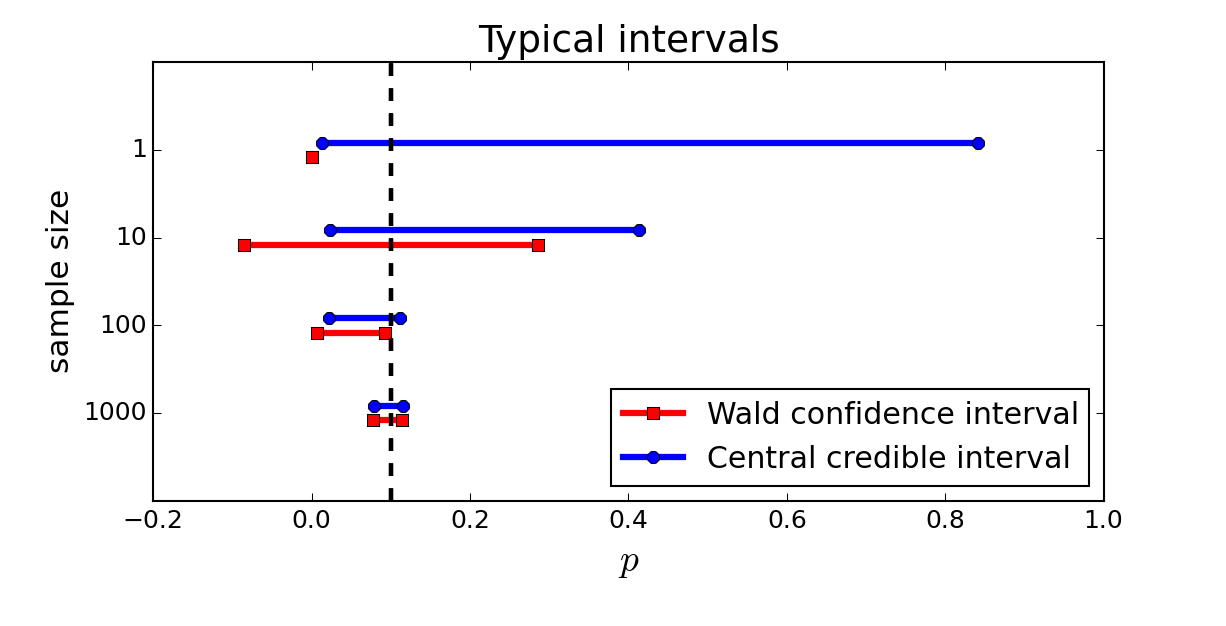
\includegraphics[trim=0 0 0 0, clip, width=0.85\textwidth]{code/ex3-intervals.png}
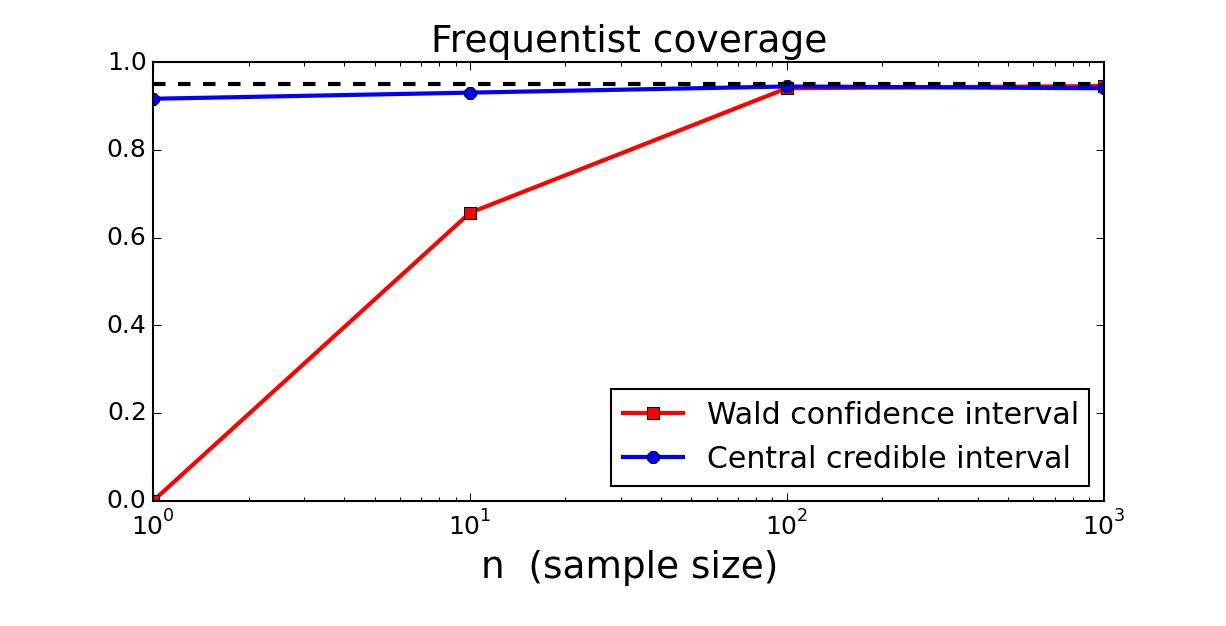
\includegraphics[trim=0 0 0 0, clip, width=0.85\textwidth]{code/ex3-coverage.png}
\end{center}
\caption{Comparison of Wald-type intervals versus Bayesian credible intervals for the Bernoulli example.}
\label{figure:intervals}
\end{figure}


\end{document}

























